\chapter{局所保存則からアインシュタインの場の方程式へ}

アインシュタインの場の方程式は一行で書けるほど単純でありながら、成分に展開すると悪名高いほど厄介である。計量には多くのクリストッフェル記号が含まれ、クリストッフェル記号には計量の導関数が含まれ、曲率テンソルにはクリストッフェル記号の導関数と積の両方が含まれる。何かを解こうとする前にさえ、計算は何ページにも及ぶことがある。特定の計量に対しては、記号計算ソフトウェアがその帳簿管理を扱う賢明な方法であることが多い。

原理は計算よりもはるかに明快である。したがって、方程式を成分ごとに攻めることから始めるのではなく、重力がどのような種類の方程式を要求するのかを問う。議論はニュートンの理論から始まり、局所保存則を経て、曲率テンソルのうちエネルギーと運動量の流れおよび密度に矛盾なく等しくなりうる唯一の組み合わせを発見して終わる。本章を通じて\(c=1\)を用いる。

\section{ニュートン的な双方向の道}

重力には二つの相補的な指示がある。重力場は物質にどのように運動すべきかを告げ、物質は重力場に何であるべきかを告げる。この双方向の道はすでにニュートン力学に見て取れる。

\(\phi(\mathbf{x},t)\)をニュートンの重力ポテンシャルとする。質量\(m\)の試験体は力
\begin{equation}
 \mathbf{F}=-m\nabla\phi.
\end{equation}
を感じる。これを\(\mathbf{F}=m\mathbf{a}\)と組み合わせると試験質量が消える：
\begin{equation}
 \mathbf{a}=-\nabla\phi.
\end{equation}
これが道の第一の方向である。場が既知であれば、それはすべての自由落下体に、その質量によらずどのように加速すべきかを告げる。

逆方向はポアソン方程式
\begin{equation}
 \nabla^2\phi=4\pi G\rho,
 \qquad
 \nabla^2=
 \frac{\partial^2}{\partial x^2}
 +\frac{\partial^2}{\partial y^2}
 +\frac{\partial^2}{\partial z^2},
 \label{eq:poisson}
\end{equation}
である。ここで\(\rho(\mathbf{x},t)\)は単位体積あたりの質量である。因子\(4\pi\)は\(G\)の定義に繰り込むこともできるが、それは別の場所で再び現れるだけである。式~\eqref{eq:poisson}は、物質の分布がポテンシャルの源であることを述べている。

全質量\(M\)の球対称な物体に対して、外部解は
\begin{equation}
 \phi(r)=-\frac{GM}{r}.
 \label{eq:newton-potential}
\end{equation}
である。密度は中心付近に集中していても、一様に広がっていても、表面に向かって滑らかに減少していてもよい。球対称性と全質量だけが、外部解が記憶するすべてである。物質の外部では\(\nabla^2\phi=0\)であり、\(1/r\)を微分すると逆二乗の力が得られる。外部のみに関心があるならば、源を点に縮めて、その点を除くどこでも同じ表式を用いてよい。

\begin{classroomqa}
\audiencequestion{球対称体の内部で密度は一定でなければならず、その境界で不連続にゼロへ跳ぶのであろうか。}
\lecturerresponse{いいえ。この議論のためには球対称でなければならないが、一定である必要も、跳ぶ必要もない。滑らかにゼロへ減少してもよい。それらの内部の詳細はいずれも外部ポテンシャルを変えず、外部ポテンシャルは全質量のみに依存する。
\lecturetimestamp{00:09:13--00:09:37}}
\end{classroomqa}

この場の定式化は、遠く離れた質量間の直接的な力よりも局所的に見えるが、ニュートン重力には依然として瞬時の遠隔作用が含まれている。源を動かせば、ニュートンポテンシャルはいたるところで同時に変化する。一般相対性理論は、力の法則だけでなく、その瞬時の応答も置き換えなければならない。

\section{弱場の手がかり、まだ方程式ではない}

第一の指示の相対論的版はすでに知られている。時空計量が与えられれば、自由落下粒子は時空測地線に従う。次に必要なのは、ポアソン方程式の相対論的置き換え、すなわち物質が計量を決定する指示である。

シュヴァルツシルト幾何は手がかりを与える。その時間-時間成分は
\begin{equation}
 g_{00}=1-\frac{2GM}{r}.
\end{equation}
である。式~\eqref{eq:newton-potential}を用いると、これは
\begin{equation}
 g_{00}=1+2\phi.
\end{equation}
となる。したがって、
\begin{equation}
 \nabla^2g_{00}=2\nabla^2\phi=8\pi G\rho.
 \label{eq:weak-mnemonic}
\end{equation}

式~\eqref{eq:weak-mnemonic}は割り引いて受け取らなければならない。それは記憶の補助であり、アインシュタインの方程式ではない。それは計量の特別な成分と非相対論的な源を用いている。それでもなお、それは我々が求めている質感を示している。一方の側に物質密度、他方の側に幾何の二階導関数である。それはポアソン方程式から共変な場の方程式への粗い橋である。

右辺には今やより注意深い検討が必要である。相対論的単位では質量はエネルギーであるから、\(\rho\)はまずエネルギー密度として理解されるべきである。しかしエネルギー密度は完全な相対論的対象ではない。それに何が伴うかを見るために、より単純な保存量から始める。

\section{電荷密度、電流、局所保存則}

\(Q\)を電荷とし、\(\sigma\)を電荷密度とする：
\begin{equation}
 \sigma=\lim_{\Delta V\to0}\frac{\Delta Q}{\Delta V}.
\end{equation}
密度は、ある瞬間に小さな空間体積をどれだけの電荷が占めるかを問う。電流は異なる問いを問う。空間に無限小の向き付けられた窓を置き、単位面積あたり単位時間あたりどれだけの電荷がそれを横切るかを数える。三つの可能な向きが空間的電流成分\(J^i\)を与える。

次元の比較は示唆に富む。電荷密度は電荷を3つの空間的長さで割ったものである。電流は電荷を2つの空間的長さと1つの時間間隔で割ったものである。\(c=1\)のとき、時間と長さは同じ単位をもつので、密度と電流は一致する次元をもつ。それらは4元ベクトルとしてまとまる：
\begin{equation}
 J^\mu=(J^0,J^1,J^2,J^3),
 \qquad J^0=\sigma.
\end{equation}

電荷の保存は、宇宙の全電荷が一定に保たれるというだけの主張ではない。それは局所的である。電荷が教室から消えて、瞬時にアルファ・ケンタウリに再び現れることはありえない。電荷がある領域から出ていくならば、その領域の境界を横切らなければならない。小さな箱について、内部の電荷の減少はその壁を通って外へ出る流束に等しい。ガウスの定理により
\begin{equation}
 \dot{\sigma}+\nabla\cdot\mathbf{J}=0,
\end{equation}
あるいは、総和規約を用いれば、
\begin{equation}
 \partial_\mu J^\mu=0.
 \label{eq:charge-continuity}
\end{equation}
曲がった座標では、対応するテンソル方程式は共変微分を用いて書かれる：
\begin{equation}
 D_\mu J^\mu=0.
\end{equation}
共変微分の目的は飾りではない。それはこの主張を任意の座標系で意味のあるものにする。

\section{なぜエネルギーと運動量には2つの添字が必要なのか}

電荷それ自体は不変である。相対運動する観測者たちは電子の電荷について一致するが、電荷密度や電流については一致しない。運動する観測者はローレンツ収縮した体積を見て、別の観測者が静止した電荷を見るところで電荷の風を見るかもしれない。したがって、全電荷は変わらないにもかかわらず、密度と電流は基準系の変更の下で混ざり合う。

エネルギーと運動量はより複雑である。それらの総量でさえ基準系に依存する。ある観測者は静止した粒子を見て、その静止エネルギーのみを担い、空間的運動量をもたないかもしれない。そばを通り過ぎる別の観測者は、運動エネルギーと運動量の両方を見る。これら4つの量は運動量4元ベクトルをなす：
\begin{equation}
 P^\nu=(P^0,P^1,P^2,P^3),
 \qquad P^0=E.
\end{equation}
各成分\(P^\nu\)は局所的に保存される。したがって各成分は密度と流れの両方をもつ。1つの添字は保存される量を特定し、2つ目の添字は密度か流れの方向かを特定する。

エネルギーから始めよう。その密度は\(T^{00}\)である。エネルギーは窓を横切ることもできるので、\(T^{0i}\)は\(x^i\)方向へのエネルギーの流れである。次に運動量の\(i\)成分を取ろう。その密度は\(T^{i0}\)であり、\(x^j\)方向へのその流れは\(T^{ij}\)である。この規約では：
\begin{itemize}
 \item \(T^{00}\)はエネルギー密度であり；
 \item \(T^{0i}\)は方向\(i\)へのエネルギー流束であり；
 \item \(T^{i0}\)は運動量の\(i\)成分の密度であり；
 \item \(T^{ij}\)は\(j\)に垂直な面を通る\(i\)運動量の流束である。
\end{itemize}
空間的ブロック\(T^{ij}\)は後に応力として認識されるであろう：その対角成分は圧力を含み、非対角成分はずりを記述する。

\begin{classroomqa}
\audiencequestion{\(T^{m0}(x)\)が運動量の\(m\)成分の密度と呼ばれるとき、\(x\)それ自体は位置の\(m\)成分を意味するのか。}
\lecturerresponse{いいえ。引数\(x\)は密度が評価される時空位置を表し、すべての座標を表している。添字\(m\)はどの運動量成分が数えられているかを示す。
\lecturetimestamp{00:41:07--00:41:27}}
\end{classroomqa}

各固定された\(\nu\)に対して、局所保存は連続の方程式を与える：
\begin{equation}
 D_\mu T^{\nu\mu}=0.
 \label{eq:stress-continuity}
\end{equation}
\(\nu\)の4つの値は、エネルギーについて1つ、運動量について3つの方程式を与える。密度と流れはともにエネルギー運動量テンソルをなす。

\begin{figure}[htbp]
\centering
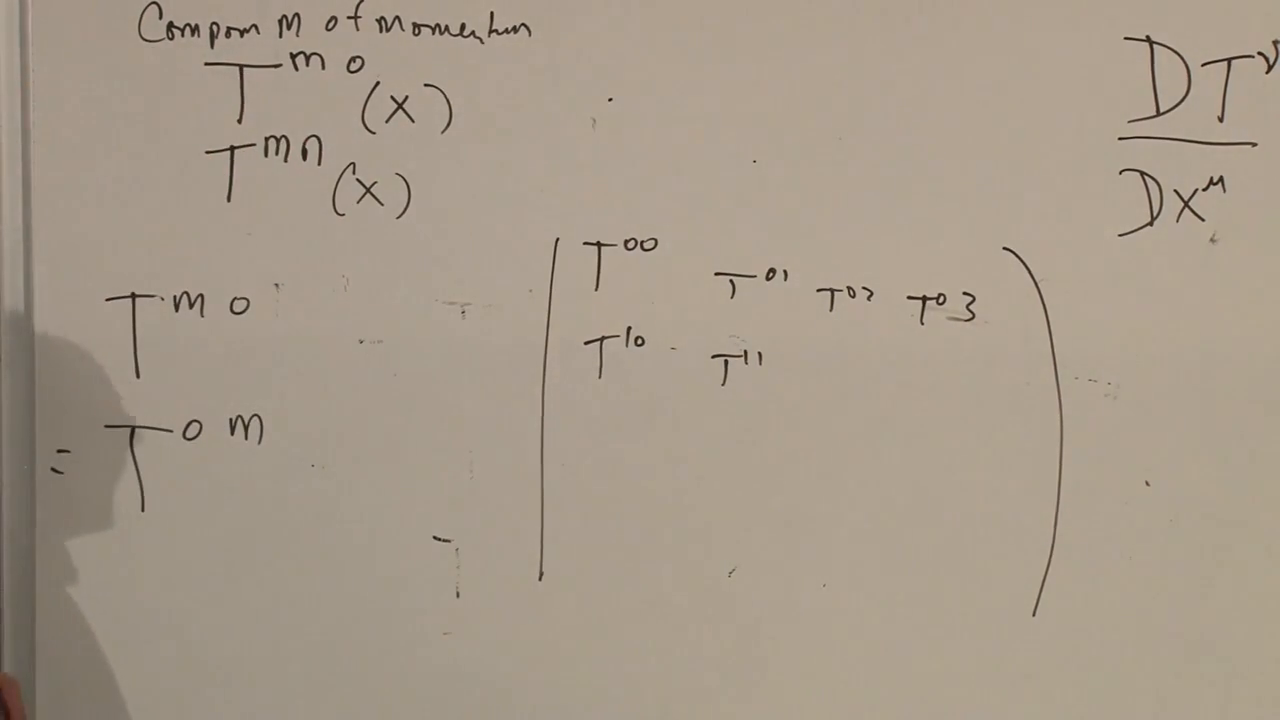
\includegraphics[width=0.84\textwidth]{lecture_09_figure_02.png}
\caption{黒板上で発展しつつあるエネルギー運動量配列。最初の添字はエネルギーまたは運動量成分を選び、2番目の添字は密度または流れを選ぶ。}
\lectureframe{00:44:30}
\end{figure}

完全な配列は
\begin{equation}
 T^{\mu\nu}=
 \begin{pmatrix}
 T^{00}&T^{01}&T^{02}&T^{03}\\
 T^{10}&T^{11}&T^{12}&T^{13}\\
 T^{20}&T^{21}&T^{22}&T^{23}\\
 T^{30}&T^{31}&T^{32}&T^{33}
 \end{pmatrix}.
\end{equation}
相対論的力学と場の理論のさらなる定理により、重力に関連する応力エネルギー・テンソルは対称となる：
\begin{equation}
 T^{\mu\nu}=T^{\nu\mu}.
 \label{eq:stress-symmetry}
\end{equation}
特に、エネルギー流束と運動量密度は、反対側から見た対応する非対角成分である。対称性により、方程式~\eqref{eq:stress-continuity}をよく知られた形で書くこともできる：
\begin{equation}
 D_\mu T^{\mu\nu}=0.
 \label{eq:stress-conservation}
\end{equation}

\begin{classroomqa}
\audiencequestion{なぜ電荷電流は1つの添字しか必要としなかったのに、エネルギー運動量は余分な添字を獲得したのか。}
\lecturerresponse{電流の添字はすでに密度と流れの方向を区別している。保存される電荷はスカラーであるため、電荷は追加のラベルを必要としない。エネルギーと3つの運動量はそれ自体が4つの成分であるので、最初の添字はどの保存量が関与しているかを示し、2番目の添字はそれが密度か流れかを示す。
\lecturetimestamp{00:45:31--00:47:24}}
\end{classroomqa}

\begin{classroomqa}
\audiencequestion{\(T^{\mu\nu}\)行列全体が対称なのか、それともエネルギー流束と運動量密度の成分だけなのか。}
\lecturerresponse{はい。行列全体が対称である。圧力や応力を含むその空間的成分の詳細な意味は、後に展開されるであろう。
\lecturetimestamp{00:47:32--00:47:54}}
\end{classroomqa}

したがって、エネルギー密度はより大きな対象のほんの一角にすぎなかった。重力の源は\(T^{00}\)だけでは首尾一貫して記述できず、完全なテンソルを含まなければならない。

\section{一つの法則は一つの成分を選び出せない}

テンソル方程式が必要であることは、曲率の計算を一切行わずに理解できる。\(A_i\)と\(B_i\)をベクトルとし、ある提案された法則が\(A_3=B_3\)だけを述べているとしよう。その等式がすべての回転した座標系で成り立つなら、第三軸を第二軸へ回転させる。同じ法則はそのとき\(A_2=B_2\)を述べ、さらに別の回転から\(A_1=B_1\)が得られる。座標系に依存しない法則とは、実はベクトル方程式
\begin{equation}
 A_i=B_i.
\end{equation}
であった。

ローレンツ変換は同じ議論を時間へ拡張する。\(A^0=B^0\)がすべての慣性系で成り立つなら、ブーストは時間成分を空間成分と混ぜ合わせ、完全な方程式\(A^\mu=B^\mu\)を要求する。優れた相対論的法則は、同じ型のテンソルを等置しなければならない。

ニュートン的な記憶法は\(T^{00}\)を特別扱いしたが、相対論的方程式は
\begin{equation}
 G_{\mu\nu}=8\pi G\,T_{\mu\nu},
 \label{eq:field-schematic}
\end{equation}
の形をとらなければならない。ここで記号\(G_{\mu\nu}\)は、最初は単なるプレースホルダーにすぎない。その要求される性質は今や明らかである：
\begin{enumerate}
 \item 対称な二階テンソルでなければならない；
 \item 物質からではなく計量から作られなければならない；
 \item 計量の二階導関数を含むべきである；
 \item その共変的発散は消えなければならない。
\end{enumerate}
最後の条件は式~\eqref{eq:stress-conservation}から従う。

\section{曲率テンソルの中を探す}

クリストッフェル記号は計量の一階導関数を含む：
\begin{equation}
 \Gamma^\sigma_{\tau\nu}
 =
 \frac12 g^{\sigma\delta}
 \left(
 \partial_\tau g_{\delta\nu}
 +\partial_\nu g_{\delta\tau}
 -\partial_\delta g_{\tau\nu}
 \right).
 \label{eq:christoffel}
\end{equation}
これらはテンソルではないので、それ自体で左辺を与えることはできない。リーマン曲率テンソルはテンソルである：
\begin{equation}
 R^\rho{}_{\sigma\mu\nu}
 =
 \partial_\mu\Gamma^\rho_{\nu\sigma}
 -\partial_\nu\Gamma^\rho_{\mu\sigma}
 +\Gamma^\rho_{\mu\lambda}\Gamma^\lambda_{\nu\sigma}
 -\Gamma^\rho_{\nu\lambda}\Gamma^\lambda_{\mu\sigma}.
 \label{eq:riemann}
\end{equation}
その最初の二つの項は計量の二階導関数を含み、最後の二つの項は一階導関数の積を含む。これはまさにニュートン方程式が示唆する微分階数である。

困難は添字構造にある。\(R^\rho{}_{\sigma\mu\nu}\)は四つの添字をもつのに対し、\(T_{\mu\nu}\)は二つである。適切な上付き添字と下付き添字を縮約するとリッチテンソルが得られる：
\begin{equation}
 R_{\mu\nu}=R^\lambda{}_{\mu\lambda\nu}.
 \label{eq:ricci}
\end{equation}
他の見かけ上の縮約は、リーマンテンソルの対称性のために消えるか、符号と添字の規約を除いて同じ対象を再現するかのいずれかである。リッチテンソルは対称であるが、完全なリーマンテンソルよりも情報が少ない：リッチテンソルが消えてもリーマンテンソルは非零でありうる。

\begin{classroomqa}
\audiencequestion{リーマンテンソルの二つの下付き添字を単純に縮約することはできないのか。縮約には一つの共変添字と一つの反変添字が必要ではないのか。}
\lecturerresponse{そのとおり。まず逆計量で添字を上げる必要があり、あるいは同等に、縮約に\(g^{\mu\nu}\)を含めなければならない。\(R^\lambda{}_{\mu\lambda\nu}\)と書けば、必要な上付き・下付きの対が明示される。
\lecturetimestamp{01:00:09--01:00:33}}
\end{classroomqa}

リッチテンソルをさらに縮約すると曲率スカラーが得られる：
\begin{equation}
 R=g^{\mu\nu}R_{\mu\nu}.
 \label{eq:ricci-scalar}
\end{equation}
このスカラーに\(g_{\mu\nu}\)を掛けると、別の対称な二階テンソルが得られる。したがって、二つの自然な候補が見つかった：
\begin{equation}
 R_{\mu\nu},
 \qquad
 g_{\mu\nu}R.
\end{equation}

\begin{figure}[htbp]
\centering
\includegraphics[width=0.78\textwidth]{lecture_09_figure_03.png}
\caption{黒板に示された二つの試行的幾何学テンソル。この段階では両者とも正しい階数と微分階数をもつので、それぞれに疑問符が付く。}
\lectureframe{01:04:56}
\end{figure}

探索的な代替案は
\begin{align}
 R_{\mu\nu}&\stackrel{?}{=}8\pi G\,T_{\mu\nu},\\
 g_{\mu\nu}R&\stackrel{?}{=}8\pi G\,T_{\mu\nu}.
\end{align}
である。添字が合うというだけの理由で、どちらも受け入れてはならない。保存則がその試金石を与える。

\section{発散のテスト}

式~\eqref{eq:field-schematic}が正しいなら、
\begin{equation}
 D_\mu G^{\mu\nu}=0
\end{equation}
が恒等的に従わなければならない。なぜなら\(D_\mu T^{\mu\nu}=0\)だからである。まず曲率スカラーの候補から始める。積の法則により
\begin{equation}
 D_\mu\!\left(g^{\mu\nu}R\right)
 =
 \left(D_\mu g^{\mu\nu}\right)R
 +g^{\mu\nu}D_\mu R.
 \label{eq:product-rule}
\end{equation}
が得られる。

\begin{figure}[htbp]
\centering
\includegraphics[width=0.84\textwidth]{lecture_09_figure_04.png}
\caption{\(D_\mu(g^{\mu\nu}R)\)に共変的な積の法則を適用する。}
\lectureframe{01:07:12}
\end{figure}

計量整合性は
\begin{equation}
 D_\mu g^{\alpha\beta}=0.
 \label{eq:metric-compatibility}
\end{equation}
を述べている。これはエネルギー・運動量保存の帰結ではなく、レヴィ・チヴィタ接続の独立した幾何学的性質である。\(R\)はスカラーなので、\(D_\mu R=\partial_\mu R\)である。したがって式~\eqref{eq:product-rule}は
\begin{equation}
 D_\mu(g^{\mu\nu}R)
 =g^{\mu\nu}\partial_\mu R
 =D^\nu R,
\end{equation}
となり、これは一般には零でない。候補\(g^{\mu\nu}R\)は失敗する。

リッチテンソルに対する対応する計算はやや長い。その結果は縮約ビアンキ恒等式である：
\begin{equation}
 D_\mu R^{\mu\nu}=\frac12 D^\nu R.
 \label{eq:contracted-bianchi}
\end{equation}
したがって\(R^{\mu\nu}\)も単独では失敗する。しかし二つの失敗は、相殺に必要なまさにその比をもつ：
\begin{equation}
 D_\mu\left(
 R^{\mu\nu}-\frac12 g^{\mu\nu}R
 \right)=0.
\end{equation}
これがアインシュタインテンソルを選び出す：
\begin{equation}
 \boxed{
 G_{\mu\nu}
 =
 R_{\mu\nu}-\frac12 g_{\mu\nu}R
 }.
 \label{eq:einstein-tensor}
\end{equation}

ここで用いている仮定の範囲内で--計量から作られ、二階以下の導関数しか含まない局所的な対称二階テンソル--、この組み合わせは全体の係数と可能な計量項を除いて固定される。後者は宇宙定数の可能性であり、講義の終わり近くで再び現れる。式~\eqref{eq:einstein-tensor}に掛かる係数は、ニュートン重力との整合によって固定される。

\begin{classroomqa}
\audiencequestion{場の方程式を、候補を試しては連続の式で棄却するのではなく、もっと直接的に物理的な方法で得ることはできないでしょうか。}
\lecturerresponse{局所的な保存はすでに物理的原理です。すなわち、エネルギーと運動量は、その領域の境界を越えることなく領域から消えることはできません。重力場の作用原理からの、より簡潔な導出もあります。その作用を変分すると同じ方程式が得られますが、計算自体は短くありません。
\lecturetimestamp{01:17:14--01:18:41}}
\end{classroomqa}

\begin{classroomqa}
\audiencequestion{同じ保存則を満たす別の幾何学的な二階テンソルはあり得るでしょうか。その答えは物理的でしょうか、それとも数学的でしょうか。また、アインシュタインはそれを知っていたのでしょうか。}
\lecturerresponse{この構成の仮定の下では、その分類は数学的です。利用可能な二階微分の曲率対象はリーマンテンソルから降りてきます。先ほど試した二つの二階の候補で、関連する縮約は尽くされています。それらの発散のない組み合わせを見つけるには、やはり計算が必要です。原理は単純ですが、添字と符号を管理することが労力なのです。
\lecturetimestamp{01:18:42--01:21:44}}
\end{classroomqa}

\section{場の方程式とそのニュートン極限}

場の方程式は今や
\begin{equation}
 \boxed{
 R_{\mu\nu}-\frac12 g_{\mu\nu}R
 =
 8\pi G\,T_{\mu\nu}
 }.
 \label{eq:einstein-equation}
\end{equation}
左辺は幾何学的であり、右辺は物質、放射、およびそれらの流れを記述します。それらの共変発散はともに消えます。

因子\(8\pi G\)は発散の議論では決まりません。それは、ゆっくり動く物質を源とする弱くゆっくり変化する重力場を考え、時間-時間成分がポアソン方程式を再現することを要求することによって決まります。その領域では\(T_{00}\simeq\rho\)であり、他の成分は\(v/c\)の冪で抑えられます。幾何学的な側は、式~\eqref{eq:weak-mnemonic}で予期された二階微分の構造に帰着します。この一致が、式~\eqref{eq:einstein-equation}の規格化を正確に与えます。

この極限は、ニュートン重力が質量密度のみを源とするように見える理由も説明します。完全な理論では、\(T_{\mu\nu}\)のすべての成分が重力源となります。すなわち、エネルギー密度、エネルギーの流れ、運動量密度、圧力、そしてずれです。通常の非相対論的物質では、静止エネルギーが支配的です。相対論的物質、放射、あるいは大きな圧力をもつ系では、残りの成分を無視することはできません。

歴史的な道筋は、単一の楽な推測ではありませんでした。リッチテンソルは明白な最初の試みのように見え、余分な\(-\tfrac12g_{\mu\nu}R\)が局所保存との整合性を回復するものです。テンソル構造が固定されれば、ニュートン極限が規格化を与えます。

\section{縮約が後に残すもの}

\begin{classroomqa}
\audiencequestion{リーマンテンソルの四つの添字を二つに縮約するとき、捨て去られた情報には物理的内容があるのでしょうか。}
\lecturerresponse{はい。リッチテンソルは時空の曲率のすべてを含んではいません。源のない重力場が最も明快な例を与えます。すなわち、潮汐曲率と重力波が残る一方で、リッチテンソルは消えることができます。この縮約は、重力場のあらゆる自由度ではなく、局所的な源の方程式に直接結びついた部分を保つのです。
\lecturetimestamp{01:21:57--01:23:10}}
\end{classroomqa}

電磁気学との類推が役立ちます。マクスウェル方程式は、電荷も電流も含まない領域に波を許します。同様に、アインシュタイン方程式は\(T_{\mu\nu}=0\)である領域に非自明な幾何学を許します。ここで、そこに成り立つより単純な方程式を導出します。

\section{真空とはリッチ平坦を意味し、平坦を意味しない}

次のように置きます。
\begin{equation}
 T_{\mu\nu}=0.
\end{equation}
すると式~\eqref{eq:einstein-equation}より
\begin{equation}
 R_{\mu\nu}-\frac12g_{\mu\nu}R=0.
 \label{eq:vacuum-einstein}
\end{equation}
\(g^{\mu\nu}\)で縮約します。
\begin{equation}
 g^{\mu\nu}g_{\mu\nu}
 =\delta^\mu{}_\mu=4
\end{equation}
が四次元時空で成り立つので、トレースは
\begin{equation}
 R-\frac12(4)R=-R=0.
\end{equation}
したがって
\begin{equation}
 R=0,
 \qquad
 R_{\mu\nu}=0.
 \label{eq:ricci-flat}
\end{equation}
真空の場の方程式はリッチ平坦性です。

\emph{リッチ平坦}という言葉を\emph{平坦}で置き換えないことが不可欠です。シュヴァルツシルト外部解は、中心特異点から離れたところには物質を含まず、\(R_{\mu\nu}=0\)を満たします。しかしそのリーマンテンソルは非零であり、潮汐力は実在します。リッチ平坦性は、すべてのクリストッフェル記号と曲率成分を手計算で計算することによって、ただしその計算は厄介ですが、あるいは記号代数システムに帳簿付けをさせることによって、検証できます。特異点では古典的な表式は発散しますが、そこから離れたどこでも真空の方程式は成り立ちます。

重力波が第二の例を与えます。それらは、本物の時空の歪みを運びながら、源のない領域を伝播することができます。したがって
\begin{equation}
 R_{\mu\nu}=0
 \quad\not\Rightarrow\quad
 R^\rho{}_{\sigma\mu\nu}=0.
\end{equation}

\section{源を保つこと：トレース方程式}

講義は真空の結果でほとんど終わりますが、聴衆の一人が、源を捨て去らずに縮約を繰り返すよう求めます。

\begin{classroomqa}
\audiencequestion{同じ縮約を、\(T_{\mu\nu}\) を方程式に残したまま行うと何が導かれるか。}
\lecturerresponse{トレースはスカラー曲率をエネルギー・運動量テンソルのトレースに直接関係づけ、その関係を元に代入し直すと、場の方程式の等価なリッチテンソル形が得られる。
\lecturetimestamp{01:29:28--01:32:20}}
\end{classroomqa}

\begin{equation}
 T=g^{\mu\nu}T_{\mu\nu}.
\end{equation} を定義する。
式~\eqref{eq:einstein-equation}のトレースを取ると
\begin{align}
 R-\frac12(4)R&=8\pi G\,T,\\
 -R&=8\pi G\,T,
\end{align}
したがって
\begin{equation}
 \boxed{R=-8\pi G\,T}.
 \label{eq:trace-relation}
\end{equation}
これを場の方程式に代入し直すと
\begin{equation}
 \boxed{
 R_{\mu\nu}
 =
 8\pi G
 \left(
 T_{\mu\nu}-\frac12g_{\mu\nu}T
 \right)
 }.
 \label{eq:ricci-form}
\end{equation}

\begin{figure}[htbp]
\centering
\includegraphics[width=0.82\textwidth]{lecture_09_figure_05.png}
\caption{トレース関係と、アインシュタイン方程式の等価なリッチテンソル形。}
\lectureframe{01:32:25}
\end{figure}

\begin{classroomqa}
\audiencequestion{スカラー \(T\) には物理的意味があるのか。}
\lecturerresponse{それはエネルギー・運動量テンソルのトレースである。電磁放射に対してはゼロであり、光子のような質量のない粒子からなる理想気体についても同じである。質量をもつ物質では一般にトレースは非零である。式~\eqref{eq:trace-relation}を通じて、そのトレースがスカラー曲率を定める。
\lecturetimestamp{01:32:20--01:33:12}}
\end{classroomqa}

\section{リッチはどれだけの曲率を覚えているか}

\begin{classroomqa}
\audiencequestion{リッチテンソルとリッチスカラーについて、リーマンテンソルに対する小さなループの平行移動に匹敵するような、簡単な物理的または幾何学的描像はあるか。}
\lecturerresponse{ここでは、それに匹敵するほど透明な描像は提示しない。リーマンテンソルは、小さなループの周りの移動によって生じる回転を直接記録する。その縮約は代数的にはより簡単であるが、個々の幾何学的意味を可視化するのはより難しい。便利だからというだけの理由で、誤解を招く描像をでっち上げるべきではない。
\lecturetimestamp{01:33:14--01:34:13}}
\end{classroomqa}

縮約で失われる情報の量は次元に依存する。4次元では、リーマンテンソルはリッチテンソルには存在しない曲率情報を含む。3次元では、リーマンテンソルはリッチテンソルによって決定される。2次元では、スカラー曲率がすべての独立な曲率情報を含む。したがって4次元重力には、\(R_{\mu\nu}\) には見えない、源のない曲率自由度の余地がある。

\begin{classroomqa}
\audiencequestion{異なるリーマンテンソルが同じリッチテンソルをもちうるなら、その失われた情報は物理的にどのように現れるのか。}
\lecturerresponse{与えられた源は、それだけでは可能なあらゆる重力配置を指定しない。境界条件と初期データには重力放射を含めることができる。弱場近似では、源のある解から出発して自由な重力波を加えると考えてよい。完全な非線形理論は任意の重ね合わせを許さないが、この例は失われた情報、すなわち \(T_{\mu\nu}\) によって局所的に固定されない伝播する曲率を正しく特定している。
\lecturetimestamp{01:37:05--01:38:59}}
\end{classroomqa}

ここで二つの真空の例が噛み合う。シュヴァルツシルト幾何は質量の外側に潮汐曲率をもたらす。重力波は自由に伝播する曲率をもたらす。それぞれが非平坦のままで \(R_{\mu\nu}=0\) を満たすことができる。

\section{宇宙定数}

\begin{classroomqa}
\audiencequestion{宇宙定数のような追加の調整項はないのか。}
\lecturerresponse{宇宙定数は許される。幾何学的な側で \(g_{\mu\nu}\) の定数倍として書くこともできるし、右辺に移してエネルギー・運動量テンソルへの真空の寄与として解釈することもできる。この二つの記述は、帳簿の付け方が異なるだけで同じ方程式である。
\lecturetimestamp{01:39:01--01:40:44}}
\end{classroomqa}

宇宙定数がある場合、よく用いられる一つの規約は
\begin{equation}
 G_{\mu\nu}+\Lambda g_{\mu\nu}
 =
 8\pi G\,T_{\mu\nu}.
\end{equation}
余分な項を右辺に移すと、有効な真空応力テンソルが定義される。
\begin{equation}
 T_{\mu\nu}^{(\Lambda)}
 =
 -\frac{\Lambda}{8\pi G}g_{\mu\nu}.
\end{equation}
計量整合性により \(D_\mu g^{\mu\nu}=0\) が成り立つので、余分な項は自動的に保存則と整合する。これが、先の一意性の主張で未解決のまま残された計量項である。

\section{水星と弱場計算}

\begin{classroomqa}
\audiencequestion{アインシュタインはこの方程式を用いて水星の軌道を計算したのか、またその計算がどのように行われたかをどこで見ることができるのか。}
\lecturerresponse{アインシュタインは、シュヴァルツシルトが厳密解を与える前に研究しており、代わりに太陽の外部場に対する十分に正確な遠距離近似を用いた。太陽の半径と水星の軌道は、太陽のシュヴァルツシルト半径に比べて極めて大きいので、相対論的補正は小さい。彼はケプラー軌道から出発し、補正を摂動的に計算することができた。シュヴァルツシルトはほどなくして厳密な外部解を得て、同じ計算を系統的にした。
\lecturetimestamp{01:40:46--01:43:48}}
\end{classroomqa}

摂動論とはまさにこれである。すでに解かれている問題から出発し、小さな補正の効果を計算する。ニュートンの逆二乗則の力は閉じたケプラー楕円を生み出す。一般相対性理論はニュートンの動径方程式に小さなずれを加えるので、楕円は一周しても閉じない。その近日点は前進する。

講義は、閉じた中心力軌道の奇妙な特殊性について述べて終わる。逆二乗則の力は、ケプラー軌道を歳差なしに閉じさせるという点で例外的である。より一般には、ベルトランの定理により、すべての束縛軌道が閉じるもう一つの中心ポテンシャルとして等方調和振動子も同定される。小さな相対論的補正はそのニュートン的縮退を取り除き、水星の歳差を、本章で導出された場の方程式の観測可能な証拠へと変える。